%%%%%%%%%%%%%%%%%%%%%%%%%%%%%%%%%%%%%%%%%%%%%%%
%%%%%%%%%%%%%%%%%%%%%%%%%%%%%%%%%%%%%%%%%%%%%%%
%%%%%%%%%%%%%%%%%%%%%%%%%%%%%%%%%%%%%%%%%%%%%%%
%%%%%%%%%%%%%%%%%%%%%%%%%%%%%%%%%%%%%%%%%%%%%%%


この章では星間物質研究の未解決のサイエンス(\S \ref{c08.s1})、国際SKAサイエンスブックの紹介(\S \ref{c08.s2})、そして日本が狙うサイエンス(\S \ref{c08.s3})をまとめる。本章は日本SKAコンソーシアム星間物質科学検討班が執筆を行った。同科学検討班は長く星間物質の研究を精力的に進めてきた日本SKAコンソーシアム有志により2014年12月に結成された。結成直後で限られた準備期間しかなく、ゆえに内容に偏りがあることを特記する。検討は現在も進行中である。

%%%%%%%%%%%%%%%%%%%%%%%%%%%%%%%%%%%%%%%%%%%%%%%
%%%%%%%%%%%%%%%%%%%%%%%%%%%%%%%%%%%%%%%%%%%%%%%
%%%%%%%%%%%%%%%%%%%%%%%%%%%%%%%%%%%%%%%%%%%%%%%
\setcounter{section}{0}\section{未解決のサイエンス}
\label{c08.s1}

この節では、まず星間物質の背景知識をまとめたうえで、天の川銀河内の星間物質と天の川銀河内の星間物質の未解決な科学的課題をまとめる。

%%%%%%%%%%%%%%%%%%%%%%%%%%%%%%%%%%%%%%%%%%%%%%%
%%%%%%%%%%%%%%%%%%%%%%%%%%%%%%%%%%%%%%%%%%%%%%%
\subsection{星間物質とは}
\label{c08.s1.ss1}

\paragraph{はじめに}

星間物質(the interstellar medium, ISM)は銀河の星間空間に存在する物質である。天の川銀河を含む我々の近傍に見られる銀河の質量構成は、90\%程度がダークマターで、10\%程度が恒星、そして数\%程度がここで取り上げる星間物質である。星間物質は気体の星間ガスと固体微粒子の星間ダストで構成されている。星間物質の質量の99\%近くは星間ガスで、残りの1\%程度が星間ダストである。また星間物質中には宇宙線が透過し磁場も存在する。このような星間物質の研究は、宇宙の物質循環を理解する要である。なぜなら銀河の物質は星風や超新星爆発によって星から星間物質へ絶えず移行し、また星間物質から次世代の星さらには惑星の形成が始まるからである。星間物質の研究は、相転移や乱流、高エネルギー物理学などにも多くの知見をもたらしている。


%%%%%%%%%%%%%%%%%%%%%%%%%%%%%%%%%%%%%%%%%%%%%%%
\subsubsection{星間物質の構成要素}
\label{c08.s1.ss1.sss1}

\paragraph{星間ガスの相}

まず星間ガスの相について簡単にまとめていく。
\begin{itemize}
\item {\bf The molecular medium (MM)}\\
星間ガスの中で最も低温のガスで、星間ガスの主成分をなす水素が分子の相をなすため分子ガスや分子雲と呼ばれる。典型的な温度は巨大分子雲で20 K程度、静穏な暗黒星雲で5 K程度である。密度は分子雲外縁部では$10^2$ ${\rm cm^{-3}}$程度、分子雲コアと呼ばれる部分では$10^5$ ${\rm cm^{-3}}$を越えるところもある。水素分子(H$_{2}$)のほか、主要なものではCO、OH、NH$_{3}$、SiOなどが存在する。特にCOの様々な回転エネルギー準位からの放射は、分子ガスの存在を知り密度と温度を探るミリ波・サブミリ波の強力なトレーサーである。星形成領域や赤色巨星の周りでは、上記の他にも有機物を含む様々な星間分子が発見されており、生命の起源との関連や星間物質の化学進化に関する研究が行われている\citep{2004PASJ...56...69K,2014ApJ...791L..38S}。

\item {\bf The cold neutral medium (CNM)}\\
星間ガスの中で分子ガスほど冷たくはないが100 K弱と温度が低く、水素が中性原子状態にあるもの。冷たい中性原子ガス、または単に原子ガスや原子雲とも呼ばれる。密度は$1$--$10^3$ ${\rm cm^{-3}}$程度。主に中性水素原子(H\,\textsc{i})からなり、わずかにHeや中性炭素(C\,\textsc{i})を含む。この相のガスは観測できるほどの強い輝線を放たないため、探査が難しい。最も実績のある方法は、背景の何らかの連続放射にみられるH\,\textsc{i}の吸収線である。CNMはコンパクトな分子雲に付随するのが通例である。

\item {\bf The unstable neutral medium (UNM)}\\
中性水素原子ガスは様々な輻射過程を介する加熱と冷却の有効なエネルギー解放系である。輻射の加熱と冷却が釣り合う輻射平衡状態にて熱的に安定な相は、CNMと次項目のWNMであることが知られ、それらが非常に薄い相転移層を隔てて共存する混相系を成すことが古くから知られている\citep{1969ApJ...155L.149F,1969JETP...29..170Z}。その中間(相転移層)に当たる相がUNMと呼ばれ、実際の観測例もある\citep{2010ApJ...725.1779B}。UNMは熱的に不安定な遷移状態のため、その存在が無視される傾向にあった。しかし、この成分の重要性は特に日本の研究者が指摘している。

\item {\bf The warm neutral medium (WNM)}\\
星間ガスの中で水素が中性原子状態にあり、数千度程度でCNMより高温側の熱的安定領域にあるもの。温かい中性原子ガスと呼ばれ、原子ガスや原子雲とも呼ばれる。WNMは分子ガスよりも密度がかなり低い($\sim 0.3~{\rm cm^{-3}}$)。このWNMのトレーサーがH\,\textsc{i}の超微細構造線、いわゆる中性水素21cm輝線である。この21cm線放射が見られる局在化した領域をH\,\textsc{i}領域やH\,\textsc{i}ガスと呼ぶ。H\,\textsc{i}輝線の研究は天の川銀河の大局的な運動学の知識などをもたらしてきた。またWNMが広がった分布をしていることも、H\,\textsc{i}ガスが銀河円盤の恒星の分布をはるかに超えて広がっていることから分かる。銀河全体で見るとWNMは分子ガスと同程度か、それ以上に大きな質量を占めていると考えられている。

\item {\bf The warm ionized medium (WIM)}\\
星間ガスの中で水素が電離状態にあり、数千度から数万度にあるもの。通常、電離ガスと言えばこの成分になる。このWIMの伝統的なトレーサーはH\,\textsc{$\alpha$}輝線やN\,\textsc{ii}禁制線([N\,\textsc{ii}])であり、可視光線の研究が中心であった。近年は必要に応じて、赤外線領域の水素再結合線も使われている。WIMはその分布によって大きく2つに分けられる。1つはこれらの輝線が見られる局在化した領域でH\,\textsc{ii}領域と呼ばれ、もう1つはH\,\textsc{ii}領域より外側にあり、銀河全体に渡って広く分布している広がった電離ガス(Diffuse Ionized Gas, DIG)である。前者は密度が$10^3$ ${\rm cm^{-3}}$を越える領域もある。後者は$10^{-2}$ ${\rm cm^{-3}}$程度以下と希薄である。WIMからはfree-free電波連続波と再結合線の2つの熱的電波が観測される。

\item {\bf The hot ionized medium (HIM)}\\
星間ガスの中でも最も高温状態にある電離ガスである。WIMと区別するため高温電離ガスと呼ばれる。数100万度にも達するガスで、自由電子の熱的制動放射と高階電離した重元素イオンの輝線放射がX線領域で観測されている。また、数10万度のガスも存在している。それらの放射の観測は難しいが、中階電離した重元素イオンの吸収線によって明らかになっている。HIMは銀河ハローに存在するコロナガスとして、また超新星爆発などに付随する高温プラズマとして観測される。

\end{itemize}
本章ではこれらのうち、イオン化していない星間ガスを中心に議論する。SKAでは、H\,\textsc{i} 21cm 輝線(1420.406 MHz)をトレーサーとした中性原子ガスと、$^{16}$OH 18cm 輝線 (1612.231、1665.402、1667.359、1720.530 MHz)をトレーサーとした分子ガスが、主な調査対象となるだろう
\footnote{
$^{16}$OHの輝線は4660.242、4750.656、4765.562、6016.746、6030.747、6035.092、6049.084、7761.747、7820.125、8135.870、8189.587、13434.596、13441.4173 MHzにもある。さらに$^{17}$OHから1624.518と1626.161 MHz、$^{18}$OHから1584.274、1637.564、1639.503、1692.795 MHzなどがある。その他にCH、H$_2$CO、CH$_2$OHなどの輝線もSKAの帯域にはある。複数種の輝線を組み合わせた分析がより精密な物理量推定につながるはずである。アメリカ国立標準技術研究所 NISTの参照値(http://physics.nist.gov/cgi-bin/micro/table5/start.pl)や国際天文学連合の重要輝線リスト(http://www.craf.eu/iaulist.htm)を参照されたい。
}。

\paragraph{星間ダスト}

天の川銀河からは遠赤外線(FIR)放射が観測される。それは星間物質中に含まれる星間ダストからの熱的連続波放射と理解されている。星間ダストの主成分はC、N、O、Mg、Siなどの化合物である。星間ダスト放射は銀河円盤で強く、それはH\,\textsc{i}放射と強い相関を持つことが知られている。詳しくは銀河進化の章(\S \ref{galaxy})を参照されたい。

\paragraph{星間宇宙線と磁場}

天の川銀河からは冪則に従う電波連続線ならびに偏波連続線が観測される。それらは星間の宇宙線電子の星間磁場を介したシンクロトロン放射と理解されている。SKAでは、シンクロトロン放射やファラデー回転、輝線のゼーマン効果が、宇宙線や磁場の主要な調査方法となる。詳しくは宇宙磁場の章(\S \ref{magnetism})を参照されたい。


%%%%%%%%%%%%%%%%%%%%%%%%%%%%%%%%%%%%%%%%%%%%%%%
\subsubsection{SKAとH\,\textsc{i}観測}
\label{c08.s1.ss1.sss2}

\paragraph{H\,\textsc{i}観測}

水素は宇宙の構成物質の70 \%以上を占める宇宙の最も普遍的な基本要素である。そのうちの中性水素原子は、超微細構造遷移による波長21cmの輝線によって観測することができるだろうと、1946年オランダのvan de Hulstは予言し、1951年アメリカのParcellとEwenによって実際に検出された。それ以来、次々とH\,\textsc{i} 21cm 線を観測する電波望遠鏡が建設され、天の川銀河や系外銀河のH\,\textsc{i} 21cm線が観測されてきた。その結果、天の川銀河の構造、銀河回転速度、銀河団における環境効果など、銀河ガス円盤の様々な性質が明らかになり、それに伴い銀河進化の理解が飛躍的に進んだ。

\paragraph{H\,\textsc{i}観測の困難}

H\,\textsc{i} 21cm線は波長が長いため、高分解能観測のためには大口径望遠鏡が必要である。干渉計技術の確立に伴い高分解能観測が可能になったが、干渉計ではミッシングフラックスのために物理量とその構造の正確な解析が難しくなる。干渉計と単一鏡を組み合わせた観測や、アレシボ300 m望遠鏡のサーベイなど一部を除いて、このミッシングフラックスは本質的な問題として残されている。そもそも分解能についても、ミリ波や可視光で達成している$1''$分解能と直接比較できる観測は容易ではない。具体的には、銀河のH\,\textsc{i} 21cm線サーベイ観測を雑音レベル1 K程度で達成するには、世界最大規模の電波干渉計JVLAやGMRTを使っても観測時間が数年も必要となる。既存の望遠鏡の規模では、H\,\textsc{i} 21cm 観測が停滞を迎えるのは時間の問題である。

\paragraph{SKAとH\,\textsc{i}観測}

以上の困難な問題を打破するには一平方キロメートルの集光面積が必要であることが、1991年IAUシンポジウムにおいて英国ジョドレルバンク天文台のPeter Williams氏によって指摘された。これがSKAの原点である。当時はH\,\textsc{i}を観測するための干渉計Hydrogen Arrayと呼ばれていたが、集光面積に焦点をおきSquare Kilometre Array (SKA)と呼ばれるようになった。以下では、H\,\textsc{i}やOHなどの輝線を$1''$分解能で超広域マッピングすることがなぜキーブレイクスルーとなるか、星間物質の諸問題に触れながらまとめていく。


%%%%%%%%%%%%%%%%%%%%%%%%%%%%%%%%%%%%%%%%%%%%%%%
%%%%%%%%%%%%%%%%%%%%%%%%%%%%%%%%%%%%%%%%%%%%%%%
\subsection{天の川銀河内の星間物質}
\label{c08.s1.ss2}

%%%%%%%%%%%%%%%%%%%%%%%%%%%%%%%%%%%%%%%%%%%%%%%
\subsubsection{星間物質の多様性}
\label{c08.s1.ss2.sss1}

\paragraph{星間物質の相転移}

冒頭で紹介したとおり、星間物質は単純に温度で5-6桁の範囲に渡り、その相は実に多様である。この多様性が星間物質研究の魅力の1つとも言える。その一方で、多様な相の形成や維持、そして相転移などは、宇宙物理学的に自明ではない。これらを理解するためには、星間雲の素片で相転移に必要な物理条件(温度や密度、圧力、紫外線強度、重元素量など)を理論的・観測的に調べ明らかにする必要がある。またその相転移が、星形成などの銀河の特性にどのような影響をあたえるのかも解明していく使命がある。

\paragraph{相転移と小スケールの中性水素原子雲}

70年代後半から、クエーサーを背景電波源とした吸収線の観測により、星間H\,\textsc{i}ガスに微小スケール(数100 AU程度かそれ以下)の構造があることが示唆されていた\citep{1976ApJ...206L.113D}。そして2000年代に入り、相転移を含んだ星間ガスの進化や動的性質の理論研究に大きな進展があった\citep{2000ApJ...532..980K, 2002ApJ...564L..97K}。主に大規模な数値シミュレーションが可能となり、十分な精度を得られるようになったからである。最近では、非常に高分解能の3次元磁気流体シミュレーションが達成されている\citep{2012ApJ...759...35I,2012ApJ...744...71I}。この研究では、頻繁に発生する超新星爆発によって発生した衝撃波を星間物質に考慮する。するとその衝撃波による圧力上昇がWNMに相転移を促し、熱的不安定なUNMを経て、小スケールのCNMの中性水素原子雲を普遍的に形成した(図\ref{c08.s1.ss2.f1})。この形成された小スケールのCNMは、星形成の現場となる分子雲の形成素片として極めて重要である。さらにこの研究では、形成された中性水素原子雲が若い超新星残骸と相互作用することによって、宇宙線加速を促進したり、宇宙線との相互作用によるガンマ線放射を通した宇宙線のプローブとしての役割を果たすなど、星間媒質で重要な役割を担っていると分かった。

\paragraph{WNM--CNM相転移の観測}

星間ガスにWNMとCNMの2つの相が存在することは、観測的にも十分知られている。しかし、衝撃波がWNMに相転移を促すということの観測的検証は未だ発展途上である。まず、理論研究において相転移に必要だった物理条件が、実際の星間物質で典型的に成り立っていることを観測的に詳細に立証することが必要である。次にその理論的予言としての小スケールの中性水素原子雲を、角度分解して観測的に見つけることが必要である。もしSKAでそれらが果たせれば、相転移ならびに分子雲形成のメカニズムの解明に向けて大きく前進するだろう。それは$1''$分解能を達成する100 kmクラスの基線長を持った、SKAという大望遠鏡でなければ達成することはできない。さらに細かい角度を分解する場合は、SKAのコア局とリモート局とを結んだVLBI観測を実現し、背景にある多数のクェーサーを利用して手前にある中性水素ガス塊を吸収線として検出する手法も考えられる\citep{1996MNRAS.283.1105D}。日本ではさらに、野辺山45m鏡やALMAといった、高感度ないし高分解能を誇る電波望遠鏡を利用できる利点を生かし、SKAで形成されたばかりの分子ガスを検出することで、比較研究することもできるだろう。

\paragraph{相転移に伴う雲の構造形成}

星間物質はしばしばフィラメント、ループ、そしてシェル状の構造をとり、フィラメントの分裂が高密度分子雲コアや原始星の形成メカニズムとして考えられている。このような構造の成因として、磁場や衝撃波が介在していると考えられている。しかし詳しいことは未だにわかっていない。前述の理論研究\citep{2012ApJ...759...35I}では、WNMが相転移する過程ではフィラメント状やクランプ状の微小構造のCNMが形成されると予言するが、観測された例は未だほとんどない。それが本当にないのか、あるが感度の問題で未検出なのか、その存在の有無や頻度をはっきりさせる必要がある。

\paragraph{CNM--MM相転移}

CNMからMMへと相転移する過程にも課題がある。CNMからMMへの相転移の程度はH\,\textsc{i}とH$_{2}$の存在比などで定量化される。銀河の大局的な性質として、この比は銀河の半径と強い逆相関があることが知られている\citep{1995A&A...304....1H}。この比は他の一般的な化学進化と同様に、星間圧力、紫外線輻射強度、金属量などの物理条件に依存する。とりわけH\,\textsc{i}とH$_{2}$の相転移では、圧力のわずかな増加で大きくH$_{2}$へ相転移し、放射強度のわずかな増加で大きくH\,\textsc{i}へ相転移する\citep{1993ApJ...411..170E}。H\,\textsc{i}とH$_{2}$の質量を直接観測できれば、CNMからMMへの相転移の程度を如実に描き出すことができるだろう。理論モデルと照らしあわせて、物理条件を推定することもできる。ただし、H$_{2}$の量をCO輝線の観測から推定する従来の方法には問題が知られているため(ダークガス問題)、その解決が求められる。間接的には、圧力などの物理条件の観測値を理論モデルに代入し、H\,\textsc{i}からH$_{2}$への相転移の程度を解明していくこともできるだろう。ただ、物理条件を観測的に得ることは簡単ではなく、例えば星間圧力とガス密度の関係には諸説ある。

\begin{figure}[tbp]
\begin{center}
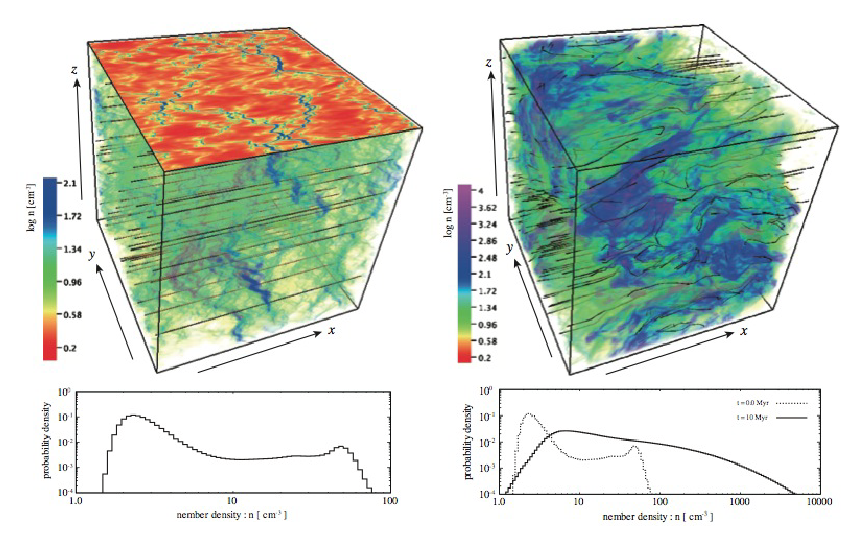
\includegraphics[width=0.8\linewidth]{ISM/c08.s1.ss2.f1.eps}
\caption{
CNM形成の3次元磁気流体シミュレーションの3次元の密度分布ならびにその確率密度分布。左は初期の熱不安定ガスの冷却時間の数倍(8 Myr)経過した後で、青い領域が熱的不安定により生まれた密度$n\gg 10~{\rm cm^{-3}}$かつ温度$T \sim 100$~KのH\,\textsc{i}雲。右は圧縮流を加えてから10 Myr経過した後で、青ならびに紫の領域が分子雲クランプを含むと目される領域($n\gg 10^2~{\rm cm^{-3}}$)。詳しくは論文を参照\citep{2012ApJ...759...35I}。
}\label{c08.s1.ss2.f1}
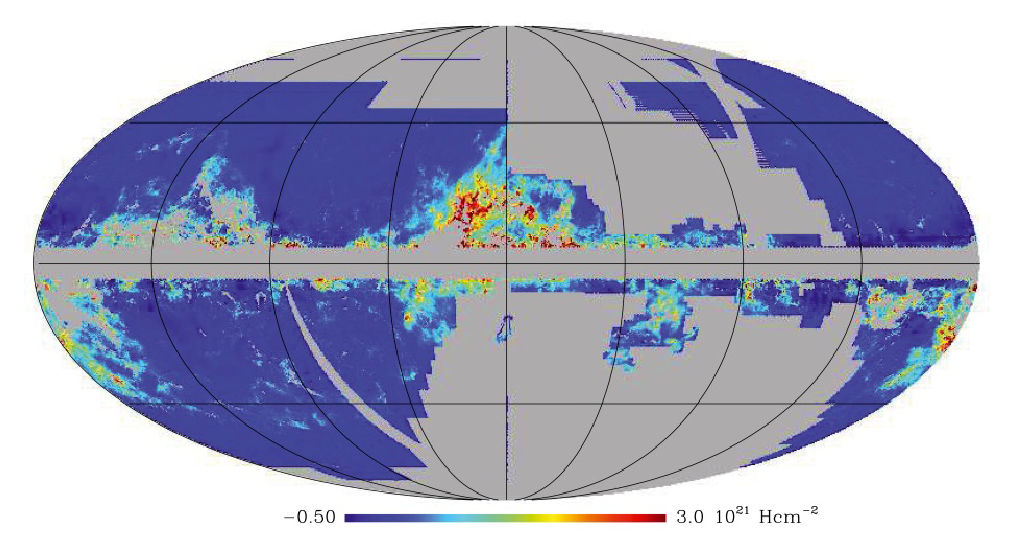
\includegraphics[width=0.8\linewidth]{ISM/c08.s1.ss2.f2.eps}
\caption{
ダークガスの銀経・銀緯全天分布。ここで言うダークガスとは、熱的ダストの光学的厚みの理論値と観測値のずれの説明に必要な中性水素原子ガス柱密度の超過量$N_{\rm H}^{\rm x}=(\tau_{\rm D}-\tau_{\rm M})/(\tau_{\rm D}/N_{\rm H})_{\rm ref}$のことである。$\tau _{\rm D}$はPlankのHFI 857 GHzデータから計算された熱的ダストの光学的厚み、$\tau _{\rm M}=(\tau_{\rm D}/N_{\rm H})_{\rm ref}N_{\rm H}^{\rm tot}$は熱的ダストの光学的厚みの理論モデル、$(\tau_{\rm D}/N_{\rm H})_{\rm ref}$はダスト放射率の参照値。$N_{\rm H}^{\rm tot}=N_{\rm H\,\textsc{i}}+N_{\rm H_2}$はトータルの水素柱密度で、$N_{\rm H\,\textsc{i}}$が中性水素原子ガスの柱密度、そして$N_{\rm H_2}=2X_{\rm CO}W_{\rm CO}$が水素分子ガスの柱密度。$W_{\rm CO}$は速度空間に積分したCO輝線強度、$X_{\rm CO}$は伝統的な$N_{\rm H_2}$/W$_{\rm CO}$変換比である。詳しくは論文を参照\citep{2011A&A...536A..19P}。
}\label{c08.s1.ss2.f2}
\end{center}
\end{figure}

%%%%%%%%%%%%%%%%%%%%%%%%%%%%%%%%%%%%%%%%%%%%%%%
\subsubsection{星間物質の乱流・磁場・宇宙線}
\label{c08.s1.ss2.sss2}

\paragraph{乱流や磁場の起源と特性}

分子雲において観測される速度分散は、ほとんどの場合熱的な速度幅よりも大きく、超音速乱流的である。低温の星間ガスも有限の電離度を持ち、磁場とよく結びついている。この乱流や磁場が分子雲コアの力学的安定性や星形成を抑制するので、これらの散逸機構が星形成のタイムスケールを決める重要な因子となる。乱流は分子雲の母体の原子ガス雲からもたらされると考えられている。SKAはスペクトル分解にも優れているので、より精密な速度分散観測が可能だろう。それを高分解に行うことで、空間的な特徴まで明らかにできるだろう。

\paragraph{星間物質と磁場の大局構造}

シンクロトロン放射やファラデー回転のSKA観測がWIMの磁場構造の情報をもたらすのに対して、WNMなど低温の星間ガスの磁場情報は、星間ダストによる偏光またはゼーマン効果(特定輝線のスペクトル分離)からもたらされる。例えばPlanck衛星は、遠赤外線領域の放射の偏光を全天に渡って観測したが、これは磁場によって整列した星間ダストの向きを表している。一方SKAはガスのゼーマン効果を測定することができ、これにより磁場の強度を調べることができる。これらを組み合わせれば、銀河磁場の大局構造や強度分布を明らかにすることができる。ゆえにSKA時代には大規模に多相の星間磁場の比較ができるだろう。

\paragraph{宇宙線の加速メカニズム}

宇宙線加速の現場として、超新星残骸がもっとも有力かつ効率的であると考えられている。その衝撃波と周囲の物質との相互作用において、磁場を増幅させる機構が重要であると考えられている。その際、星間物質の密度のムラが重要であるが、それが確かに小さな構造であることや密度の正確な定量が必要であることなど、観測的に明らかにすべき課題は多い。この問題も、SKAの高分解観測が大きなブレイクスルーとなるだろう。


%%%%%%%%%%%%%%%%%%%%%%%%%%%%%%%%%%%%%%%%%%%%%%%
\subsubsection{ダークガス問題}
\label{c08.s1.ss2.sss3}

\paragraph{ダスト質量からガス総量を求める経験則}

電波天文学の教科書に掲載されているように、H\,\textsc{i}輝線強度は柱密度に比例し、スピン温度(H\,\textsc{i}輝線に対する励起温度)には寄らないことから、H\,\textsc{i}ガスの量は正しく見積もられていると考えられてきた。しかしながら、ガンマ線の観測から見積もられたガスの相(中性原子ガスもしくは分子ガス)によらない陽子の量は、H\,\textsc{i}強度から見積もられる中性水素原子ガスの量と、COの観測から求められる水素分子ガスに含まれる水素原子の量の総和とは比例しておらず、ガスの量の不足分が近年になって明らかになってきた。この不足分はダークガスと名付けられている\citep{2005Sci...307.1292G}。また、サブミリ波帯のダスト連続波の観測\citep{2011A&A...536A..19P}からも同様の結果が示唆されている(図\ref{c08.s1.ss2.f2})。このダークガスは、COでは検出されない分子ガスの可能性の他に、ダストの性質が異なるなどの理由でガス-ダスト比が一定ではないとする説や、H\,\textsc{i}輝線が光学的に厚いためにH\,\textsc{i}輝線強度から見積もられる中性水素原子ガス量が過小評価されているとする説が提唱されている。

\paragraph{OH分子雲探査}

COでは検出されない分子ガスの解釈として、H$_2$は存在するがCOが解離されている、または低密度でCOの励起条件を満たしていない、などの可能性が議論されている。これまでは歴史的にCO分子はH$_2$と十分よく混ざっていると考えられていたが、そうでないのかもしれない。この問題は、COの代わりにOH分子をH$_2$のトレーサーとして使用することで検証できるだろう。例えばSPLASH(Southern Parkes Large Area Survey for Hydroxyl)におけるパイロット掃天観測では、OH輝線の分布はCOのそれよりも狭いと報告されている\citep{2014MNRAS.439.1596D}。しかし、空間分解能が$14'$だったことと感度による検出限界がその理由として考えられる。COと直接比較できるようにするために、CO観測で達成している$1''$分解能を実現したい。そのためには、十分な感度を与える集光面積を持ち、かつ$1''$分解能を達成する100 kmクラスの基線長を持った、SKAという大望遠鏡が不可欠である。

\paragraph{H\,\textsc{i}高分解探査}

中性水素原子ガス量の過小評価に関しては、H\,\textsc{i}輝線強度が中性水素原子ガスの柱密度に比例することを前提とした推定が誤っている可能性がある。この比例関係はH\,\textsc{i}輝線が光学的に薄い場合に近似的に成り立つもので、光学的に厚い場合は良い近似とならない。ダスト量とH\,\textsc{i}ガス量との関係を詳細に比べると、この説を支持する証拠が集まりつつある\citep{2014ApJ...796...59F,2015ApJ...798....6F}。この説を確かめる1つの方法として、従来にない高い分解能によるH\,\textsc{i}観測が期待できる。H\,\textsc{i}が光学的に厚い領域は狭い範囲に集中していることが期待され、その周囲では光学的厚さが次第に薄くなっていることが予想されるからである。この光学的厚さの空間的な遷移が観測されれば、ダークガスがH\,\textsc{i}の光学的厚さによることを強く裏付けることができよう。


%%%%%%%%%%%%%%%%%%%%%%%%%%%%%%%%%%%%%%%%%%%%%%%
%%%%%%%%%%%%%%%%%%%%%%%%%%%%%%%%%%%%%%%%%%%%%%%
\subsection{天の川銀河外の星間物質}
\label{c08.s1.ss3}

%%%%%%%%%%%%%%%%%%%%%%%%%%%%%%%%%%%%%%%%%%%%%%%
\subsubsection{銀河進化と分子雲形成過程}
\label{c08.s1.ss3.sss1}

\paragraph{分子雲形成過程とH\,\textsc{i}観測}

星形成の舞台である分子雲の寿命については論争が絶えないが、銀河進化の時間スケール(例えばGyr)よりは短いと考えられるため、銀河進化の時間スケールでは分子雲が絶えず形成されていると言える。銀河進化を決定的に左右する星形成過程を理解するためには、分子雲形成過程を宇宙論的時間で理解することが必須である。恒星進化と星間物質の変遷を繋いでできている宇宙の物質循環を考えると、電離ガスから中性原子雲が形成され、中性原子雲から星間分子雲が形成される過程は、残された最後のミッシング・リンクである。SKAによるH\,\textsc{i}観測は、ここを直接解明できる重要な地位を占める。

\paragraph{分子雲形成過程の現状の理解}

現在の分子雲形成過程についての理論的研究は2000年頃に始まり\citep{1999A&A...351..309H, 2000ApJ...532..980K}、ようやくその全体像を記述するシナリオが描けるようになってきた。それによると、膨張する電離領域や超新星爆発により形成されたバブルの表面で、H\,\textsc{i}雲は普遍的に形成される。しかし、$\mu$G程度の磁場を含む標準的な星間媒質においては、分子雲はバブルによる度重なる圧縮を経て形成されることになる\citep{2008ApJ...687..303I, 2009ApJ...704..161I, 2012ApJ...759...35I}。つまり、分子雲の形成時間はバブルの膨張時間である百万年を優位に超える長い時間スケールになることが提案されている\citep{2013ASPC..476..369I}。ゆえに天の川銀河にとどまらず、様々な星形成の特徴を持つ系外銀河へを目を向けることも重要である。


%%%%%%%%%%%%%%%%%%%%%%%%%%%%%%%%%%%%%%%%%%%%%%%
\subsubsection{系外銀河のH\,\textsc{i}サーベイ}
\label{c08.s1.ss3.sss2}

\paragraph{系外銀河のH\,\textsc{i}サーベイの重要性}

H\,\textsc{i}ガスから分子雲がどのようにして形成されているかを観測的に調べ、星間媒質の物質循環を銀河スケールで理解することは、星形成を理解し、星形成史にもとづく銀河進化を理解するためには必須である。系外銀河ならface-on geometryを活かして分子雲の空間構造とH\,\textsc{i}の空間分布とを直接天球上で比べることが可能となる。これは天の川銀河ではできず、face-on系外銀河のH\,\textsc{i}分布の詳細なサーベイによってのみ可能である。また、この輝線観測に加え、連続波の偏波観測も重要である。なぜなら長波長の電波連続波は多くの場合、宇宙線からのシンクロトロン放射を見ているので、高エネルギー電子の分布及び磁場の向きの分布を測定できるからである。偏波観測から得る磁場構造は、H\,\textsc{i}ガスやCOによる分子ガスの空間構造と比較すべきものであり、また前述のH\,\textsc{i}雲から分子雲への相転移の程度を決める重要な物理変数である。その観測はSKAによって最も能率的に進めることができる。

\paragraph{系外銀河のH\,\textsc{i}サーベイの現状}

すでに一部の円盤銀河においては分子雲の詳細サーベイが行われているので\citep{2013ApJ...779...42S}、詳細な円盤銀河中のH\,\textsc{i}雲分布及び宇宙線・磁場構造を得ることができれば、それらのデータと組み合わせることで、円盤銀河における星間媒質のダイナミックスに対する初めての本格的な研究が可能となるだろう。円盤銀河の渦状腕構造はH\,\textsc{i}雲及び分子雲が集中している所なので、渦状腕構造の起源に迫ることも可能である。Face-on円盤銀河のサーベイのみならず、edge-on銀河の詳細マッピングと組み合わせることで、銀河円盤の垂直方向の星間媒質の構造の理解も同時に進められる。これも銀河円盤における物質循環を理解するためには重要である。

\paragraph{大小マゼラン銀河}

我々の銀河の伴銀河である大小マゼラン銀河(LMC、SMC)において見られる星形成は、現在我々の銀河で一般的にみられるそれとは大きく異なっている。星間物質も金属量の少ない環境であり、我々の銀河の過去の状況に近いのでないかと考えられている。分子雲探査はNANTEN望遠鏡が全面をサーベイし、ALMAでのフォローアップ観測も進んでいる。H\,\textsc{i}ガスはATCAが40秒角のマップを公開しているが、多くのシェル状構造が検出されるなど興味深い幾何学的構造を示す。大小マゼラン銀河の分子雲は空間分解して我々の銀河の分子雲と比較できる数少ないターゲットであり、環境の違いを議論する絶好の対象である。LMCはほぼface-onなので、分子雲の空間構造とH\,\textsc{i}の空間分布とを直接天球上で比べることも可能である。

%%%%%%%%%%%%%%%%%%%%%%%%%%%%%%%%%%%%%%%%%%%%%%%
\subsubsection{系外銀河のダスト--ガス比}
\label{c08.s1.ss3.sss3}

\paragraph{ダスト--ガス質量比の観測}

星間物質中のダスト質量とガス質量との関係は単純ではない。なぜなら銀河の星形成によって重元素量が増え、化学進化が進むことによって、ダスト量は刻々と進化してゆくからである。ところが、ダスト--ガス質量比の関係する従来の研究の多くでは、天の川銀河のような成長の進んだ銀河で見られる経験則が用いられてきた。あらゆる宇宙年齢、様々な重元素量や形態の銀河に一つの経験則を適用する、かなり無理のある議論である。このように議論の土台が危ういのは明確にもかかわらず、ALMAによるダスト放射の光度をもとにダスト質量を算出し、ダスト-ガス質量比を介して全ガス質量に換算するという議論が広く用いられるようになってきている。この土台となっているダスト--ガス質量比関係は観測によって検証されるべきものである。実際にHerschelなどの観測から、現在仮定されている関係が低金属量で破れていることが明らかになってきた\citep{2014A&A...563A..31R}。

\paragraph{ダスト--ガス質量比のモデル化}

\begin{figure}[tbp]
\begin{center}
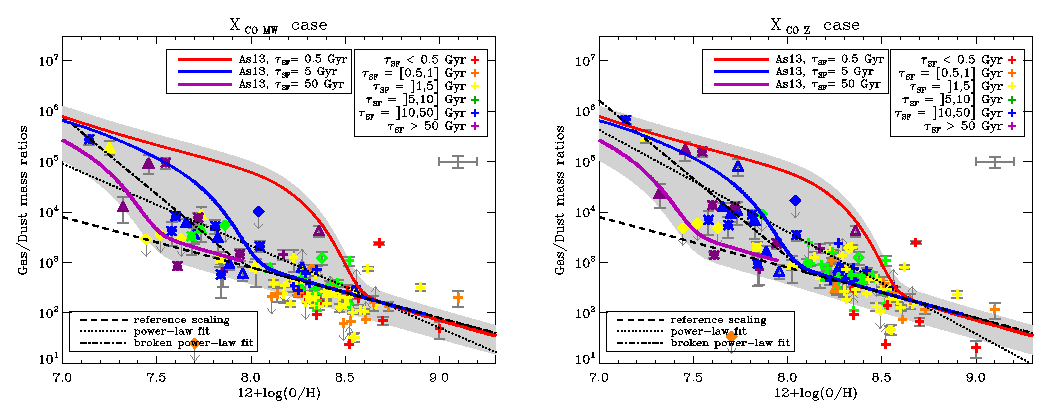
\includegraphics[width=1.0\linewidth]{ISM/c08.s1.ss3.f1.eps}
\caption{
さまざまな金属量の銀河におけるダスト--ガス質量比。シンボルはHerschelによる観測\citep{2014A&A...563A..31R}。太実線はモデルの予言\citep{2013MNRAS.432..637A}。シンボルのカラーはSEDフィットから算出した星形成の指数的減衰のタイムスケール$\tau_{\rm SF}$。モデルの線のカラーは$\tau_{\rm SF} = 0.5$~Gyr: 赤、5~Gyr: 青、0.5~Gyr: 紫を表している。
}\label{c08.s1.ss3.f1}
\end{center}
\end{figure}

ダスト--ガス質量比関係の理論的研究は80年代から行われていたものの、定式化が非常に複雑なこともあって、信頼できる枠組みができたのはごく最近のことである\citep{2013MNRAS.432..637A, 2013EP&S...65..213A, 2014MNRAS.440..134A}。この理論モデルでは、100億年以上にわたる全銀河年齢での銀河のガス量とダスト量を、化学進化と整合的に解くことができる。図\ref{c08.s1.ss3.f1}には観測結果との比較を示す。この理論モデルの重要な結論は、ダスト-ガス比が重元素量の強い非線型関数となっていることである。これは、ダスト粒子が超新星やAGB星から供給される効果と、シードになる小さな粒子に星間物質中の重元素が吸着されて成長する効果を取り入れることではじめて正しく理解された現象であり、現在の天の川銀河や遠方クェーサーでみられる豊富なダスト量はこの効果なしで説明することは不可能である。このように、新しい理論は強力な予言力を持っているものの、これが完成形ではない。取り入れるべき星間物理過程も将来改訂されるであろうし、銀河の進化に関する新しい知見も付け加えられることは間違いない。すなわち、理論モデルも詳細な直接観測によって検証されるべきである。SKAはこの関係の検証にも大きく貢献することは明らかである。

